\documentclass[10pt]{article}

\usepackage[margin=0.78in]{geometry}
\usepackage{amsmath,amssymb}
\usepackage{graphicx}
\usepackage{booktabs}
\usepackage{array}
\usepackage{xcolor}
\usepackage[hidelinks]{hyperref}

\graphicspath{{../figures/}}
\setlength{\parindent}{0em}
\setlength{\parskip}{0.45em}
\renewcommand{\arraystretch}{1.12}

\newcommand{\exactE}{-29.146168109350}
\newcommand{\hvaE}{-29.037601351802}
\newcommand{\hvaF}{0.982518440088}
\newcommand{\rvbE}{-29.012072100265}
\newcommand{\rvbF}{0.978535993636}

\title{\textbf{Report 1: Initial Progress Report}\\
\large Weighted-RVB Initialization and Heisenberg-HVA Refinement\\
for a 19-Site Kagome Heisenberg Benchmark}
\author{Adel H. Al-Yoorby\\
QIntern 2026 Project qi26\_09\\
Project context: Dr. Muhammad Ahsan}
\date{July 2026}

\begin{document}
\maketitle

\section*{1. Project Idea}

This is an initial progress report, not a final research manuscript.  The goal is to test a potential no-calibration route for preparing low-energy states of a 19-site Kagome antiferromagnetic Heisenberg benchmark.  The main idea is to improve the variational state structure rather than modify the target Hamiltonian.

\textbf{Potential solution.}  Start from a physically motivated signed weighted resonating-valence-bond (RVB) state, then refine it using shallow edge-colored Heisenberg Hamiltonian variational ansatz (HVA) layers.  The target Hamiltonian remains fixed:
\[
H=\sum_{\langle i,j\rangle}(X_iX_j+Y_iY_j+Z_iZ_j).
\]
The exact fixed-sector benchmark energy for the 19-site patch is
\[
E_0=\exactE.
\]
The current preliminary no-calibration result reaches
\[
E=\hvaE,\qquad F=\hvaF
\]
at HVA depth $p=4$.

\begin{center}
\small
\fbox{19-site Kagome graph}
$\rightarrow$
\fbox{signed weighted RVB}
$\rightarrow$
\fbox{Heisenberg-HVA}
$\rightarrow$
\fbox{exact energy/fidelity check}
\end{center}

\textbf{Repository / current work link.}\\
\href{https://github.com/adoolelomani2026/qintern-kagome-hva}{https://github.com/adoolelomani2026/qintern-kagome-hva}

\textbf{One-sentence status.}  The current evidence is a finite-size proof-of-concept that weighted-RVB structure plus shallow Heisenberg-level refinement can move a dimer/RVB state close to the exact 19-site ground state, but it does not yet prove scalable or hardware-ready quantum spin liquid preparation.

\newpage

\section*{2. Background and Benchmark}

The Kagome antiferromagnetic Heisenberg model is a standard frustrated-magnetism benchmark because its geometry makes simple classical ordering difficult.  In the thermodynamic limit, this model is closely connected to quantum spin liquid physics.  Here the project uses a smaller 19-site open-boundary patch because it is still large enough to show nontrivial frustration while remaining small enough for exact fixed-$S^z$ diagonalization.

The active benchmark is the 19-site graph and bond list confirmed from the project provenance material.  The calculation is performed in the fixed sector with $n_\downarrow=9$, whose Hilbert-space dimension is
\[
\dim \mathcal{H}_{n_\downarrow=9}=\binom{19}{9}=92{,}378.
\]
This is large enough that naive full statevector work is inconvenient, but small enough for sparse diagonalization and optimized fixed-sector NumPy kernels.

\textbf{Why this benchmark is useful.}  A static dimer product is a natural starting point, but it is too rigid: it locks singlet weight onto specific bonds.  A more flexible RVB state allows many dimer coverings to interfere with signs and amplitudes.  The HVA then adds circuit-compatible two-qubit Heisenberg evolution gates:
\[
U_{ij}(\theta)=\exp[-i\theta(X_iX_j+Y_iY_j+Z_iZ_j)].
\]

\textbf{Role of calibrated-Hamiltonian work.}  The calibrated-Hamiltonian direction discussed in the project is treated as methodology context and as a source of ansatz-design clues.  In this initial no-calibration route, the Hamiltonian used for evaluation is not changed.  Instead, future work can use the information from sensitive triangles or bonds to design better circuit blocks.

\begin{center}
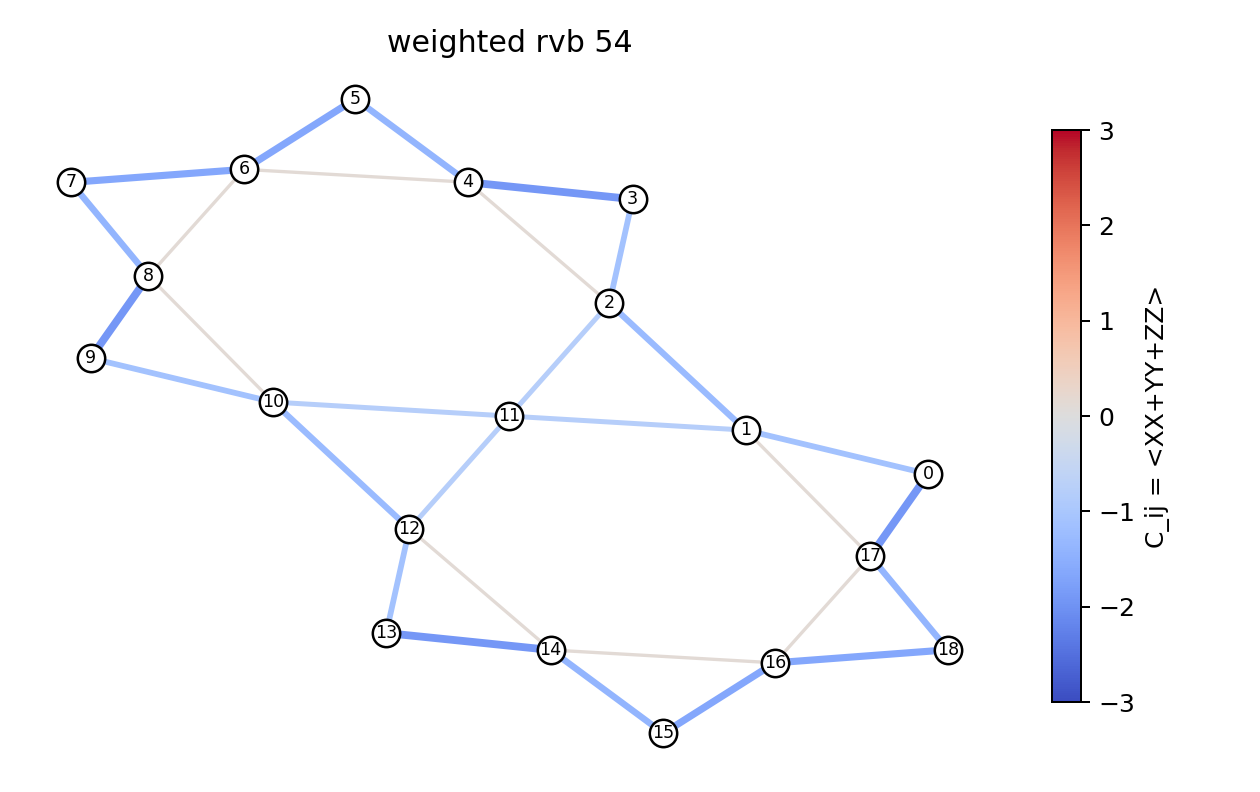
\includegraphics[width=0.78\linewidth]{bond_map_weighted_rvb.png}

\small Figure 1. Bond-correlation map for the weighted-RVB initializer.
\end{center}

\newpage

\section*{3. Current Method}

The current workflow has two main stages.

\textbf{Stage 1: weighted RVB initialization.}  The code enumerates 54 maximum dimer coverings on the 19-site graph.  Instead of taking an equal positive superposition, it solves a classical generalized eigenproblem in the dimer-covering subspace.  This produces a signed weighted-RVB state.  The equal RVB state is not enough; the signs and amplitudes are important.

\textbf{Stage 2: edge-colored Heisenberg-HVA refinement.}  The 30 graph bonds are partitioned into four disjoint edge-color groups.  Within each group, gates act on disjoint bonds and can be applied in parallel.  A depth-$p$ ansatz therefore uses only $4p$ HVA parameters:
\[
U_p=\prod_{\ell=1}^{p}\prod_{c=1}^{4}\prod_{(i,j)\in E_c}
\exp[-i\theta_{\ell,c}(X_iX_j+Y_iY_j+Z_iZ_j)].
\]
For the current best no-calibration run, $p=4$, so the HVA refinement uses 16 parameters.

\textbf{Why this is a reasonable first route.}  The ansatz is physically matched to the Hamiltonian because every two-qubit gate is a Heisenberg interaction.  It also avoids immediately relying on Hamiltonian calibration.  That keeps the scientific question clean: how far can a better initial state plus physically structured circuit layers go against the original target Hamiltonian?

\begin{center}
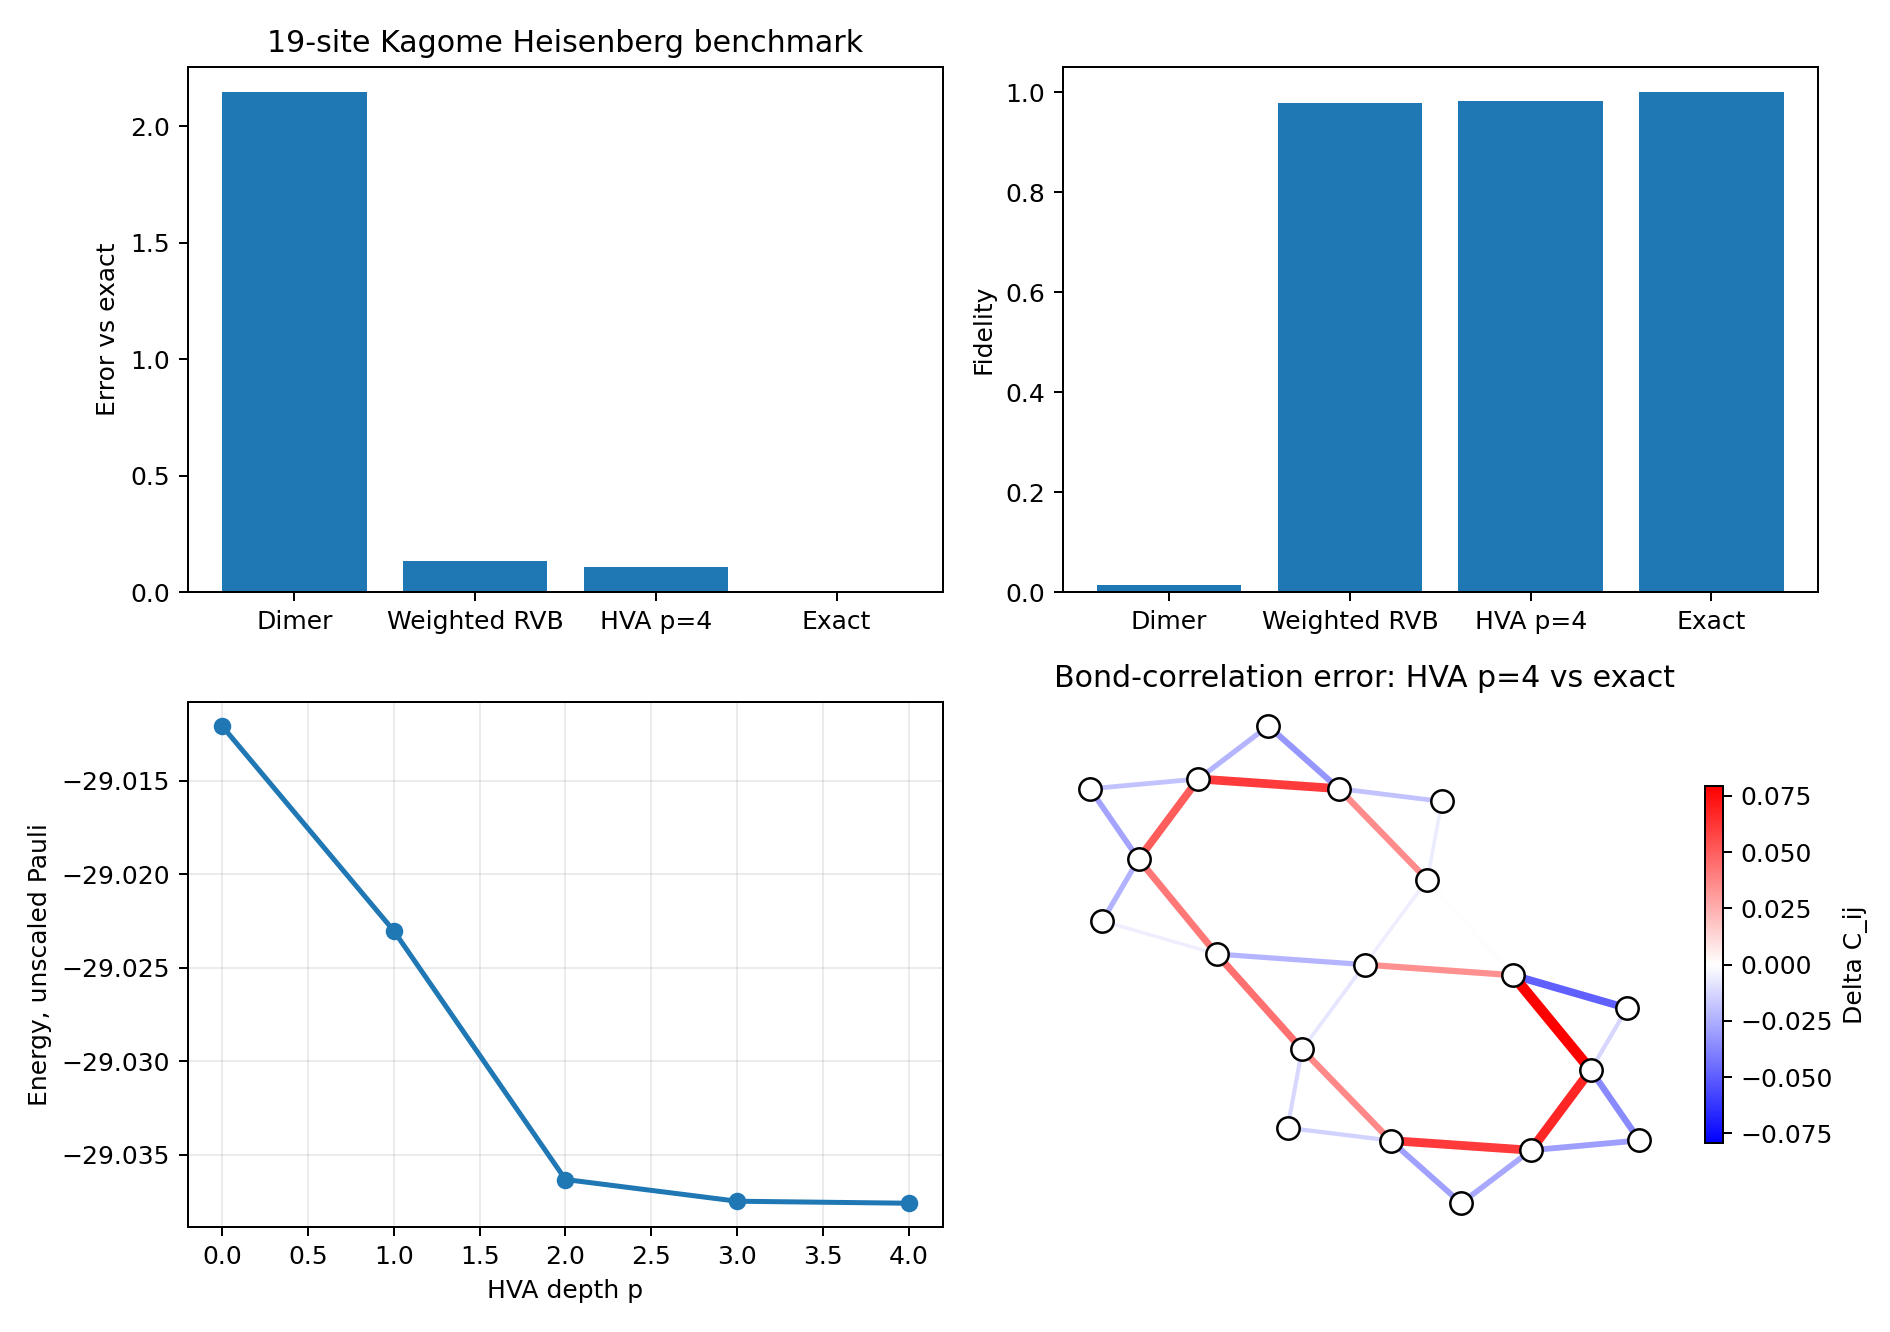
\includegraphics[width=0.82\linewidth]{one_page_summary.png}

\small Figure 2. Compact summary of the current finite-size proof-of-concept.
\end{center}

\newpage

\section*{4. Preliminary Results}

The table below summarizes the current main result in the unscaled Pauli convention.  Energy and fidelity are always measured against the same fixed target Hamiltonian and the exact 19-site ground state.

\begin{center}
\begin{tabular}{lrrr}
\toprule
State & Energy & Error vs exact & Fidelity \\
\midrule
Static dimer & -27.00000000 & 2.14616811 & 0.014241 \\
Equal RVB-54 & -26.39781307 & 2.74835504 & 0.004371 \\
Weighted RVB-54 & \rvbE & 0.13409601 & \rvbF \\
Weighted RVB + HVA $p=2$ & -29.03633182 & 0.10983629 & 0.982446 \\
Weighted RVB + HVA $p=4$ & \hvaE & 0.10856676 & \hvaF \\
Exact & \exactE & 0.00000000 & 1.000000 \\
\bottomrule
\end{tabular}
\end{center}

The static dimer state is far from the exact state.  The equal RVB state is also poor, which shows that merely superposing dimer coverings is not enough.  The signed weighted-RVB state gives the largest improvement, reaching fidelity about 0.9785.  The Heisenberg-HVA refinement then gives a smaller but useful improvement, reaching fidelity about 0.9825 at $p=4$.

\begin{center}
\begin{minipage}{0.48\linewidth}
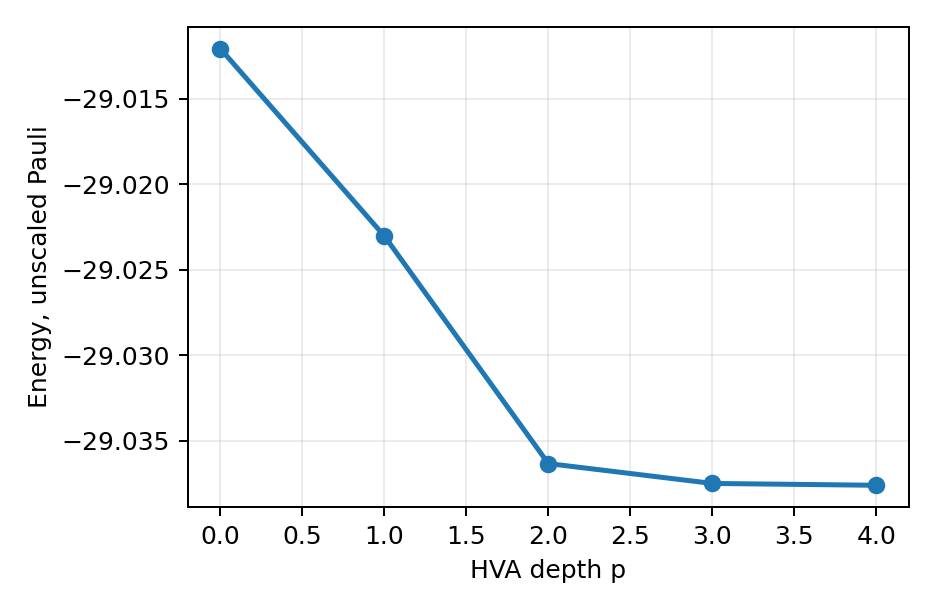
\includegraphics[width=\linewidth]{energy_vs_hva_depth.png}
\end{minipage}
\hfill
\begin{minipage}{0.48\linewidth}
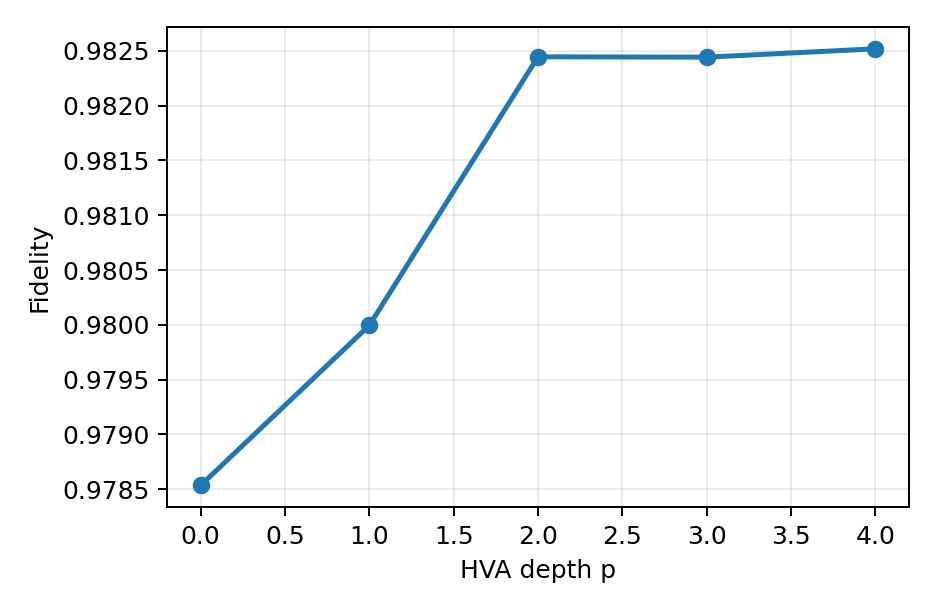
\includegraphics[width=\linewidth]{fidelity_vs_hva_depth.png}
\end{minipage}

\small Figure 3. Energy and fidelity versus HVA depth after weighted-RVB initialization.
\end{center}

\textbf{Current interpretation.}  The result is promising as a finite-size baseline.  It suggests that improving the state structure matters more than simply adding arbitrary circuit depth.  However, the remaining no-calibration energy gap is still about $0.1086$, so this is not yet a finished solution.

\newpage

\section*{5. Next Step and Limitations}

The most useful next step is not a blind depth sweep.  The controlled next experiment is calibration-informed ansatz design: use the sensitive local structures identified by calibration studies as extra circuit blocks, but keep the target Hamiltonian unchanged.  For example, add a local Heisenberg block on triangle $(6,7,8)$ or bond $(14,16)$:
\[
U_{\triangle}(\alpha)=\prod_{(i,j)\in \triangle}
\exp[-i\alpha(X_iX_j+Y_iY_j+Z_iZ_j)].
\]
This tests whether calibration information can guide circuit expressibility without becoming Hamiltonian calibration.

\begin{center}

\includegraphics[width=0.58\linewidth]{calibration_energy_vs_fidelity.png}

\small Figure 4. Calibration scans are useful as reference information and ansatz-design guidance.
\end{center}

\textbf{Limitations at this stage.}
\begin{itemize}
\item The result is finite-size only and uses a 19-site open-boundary patch.
\item The weighted-RVB initializer is obtained classically and is not yet a hardware-preparable state-preparation circuit.
\item The HVA improvement is real but modest through $p=4$.
\item No statistical robustness campaign, noise model, or hardware execution is claimed in this initial report.
\item This report should be read as a progress report and potential solution direction, not as a final proof.
\end{itemize}

\textbf{Short reference context.}  The project is motivated by Kagome Heisenberg and quantum spin liquid work such as Yan, Huse, and White (Science, 2011) and Depenbrock, McCulloch, and Schollw\"ock (PRL, 2012), and by the calibrated-Hamiltonian VQE direction in M. Ahsan, ``Utility-scale Experimental Quantum Computation with Hardware Efficient Ans\"atze and Calibrated Hamiltonian,'' \emph{ACM Transactions on Quantum Computing} (2026), doi:10.1145/3815786.

\end{document}
